\newpage
\section{Dynamic Simulation of the Arm: A Comprehensive Model for Musculoskeletal Dynamics}
The study of human mobility has benefited greatly from the development of musculoskeletal modeling, which is now a crucial tool for comprehending the dynamics of the human body. Multibody models have historically proved helpful in resolving inverse dynamic issues, particularly in the analysis of human gait and arm movement (please add paper citation for more information). The main disadvantage of these inverse dynamic techniques is the need to gather data from participants who are actively doing the required movement.

Moving away from conventional techniques, muscle-driven forward dynamics have allowed the simulation of innovative and fictional movements that would resemble impaired movements, such as those of stroke survivors. These simulations have practical applications in fields such as rehabilitation and motor control research. In \cite{IMP} the DAS allowed to test controllers and command interfaces with a human user in the loop. For this project, forward dynamics simulation will be used to test the hypothesis for EMG-inspired PD control of Functional Electrical Stimulation (FES) in stroke rehabilitation. 

A summary of the musculoskeletal dynamics, including topics like multibody dynamics, muscle contraction dynamics, and muscle activation dynamics, will be covered in this section. Then, an explanation of the forward-dynamic implicit formulation will be given. This formulation has been proven to improve the computational time required to model dynamics with only an RMS error of 0.11 degrees in joint angles when running at real-time speed for a gait simulation with a prosthetic foot and ankle \cite{IMP}.

Overall, the Dynamic Arm Simulator (DAS) offers a robust framework for the simulation of human arm movements. It is implemented as a MATLAB Mex function that contains the system dynamics and other functions, making it accessible via a MATLAB function interface, flexible, and adaptable for various applications. 

An extended overview of the DAS model is provided in the following sections.

\begin{table}[h!]
    \centering
    \caption{Nomenclature}
    \label{tab:nomenclature}
    \begin{tabular}{|l l|}
        \hline
        \multicolumn{2}{|c|}{\textbf{Nomenclature}} \\ \hline
        \textbf{$q$} & Generalized coordinates vector \\
        \textbf{$\dot{q}$} & Generalized angular velocities vector \\
        \textbf{$M(q)$} & Mass matrix \\
        \textbf{$\tau$} & Generalized forces vector/ Joint moments \\
        \textbf{$B(q,\dot{q})$} & Coriolis, centrifugal and passive forces matrix \\
        $L_M$ & Muscle-tendon length \\
        $L_{CE}$ & Muscle contractile element length \\
        $\phi$ & Pennation angle \\
        $s$ & Muscle contraction dynamics state variable \\
        $a$ & Activation state \\
       \textbf{$x$} & State vector $x = (q,\dot{q},s,a)^T$ \\
       \textbf{$u$} & Neural excitations for each muscle \\ \hline
    \end{tabular}
\end{table}
\newpage
\subsection{Structural Overview}
Links and Degrees of Freedom
\begin{itemize}
    \item \textbf{7 Links}: Includes the thorax, clavicle, scapula, humerus, ulna, radius, and hand. Figure \ref{fig:links} shows a colour-coded of the different links. 
\end{itemize}

\begin{figure}[h!]
    \centering
    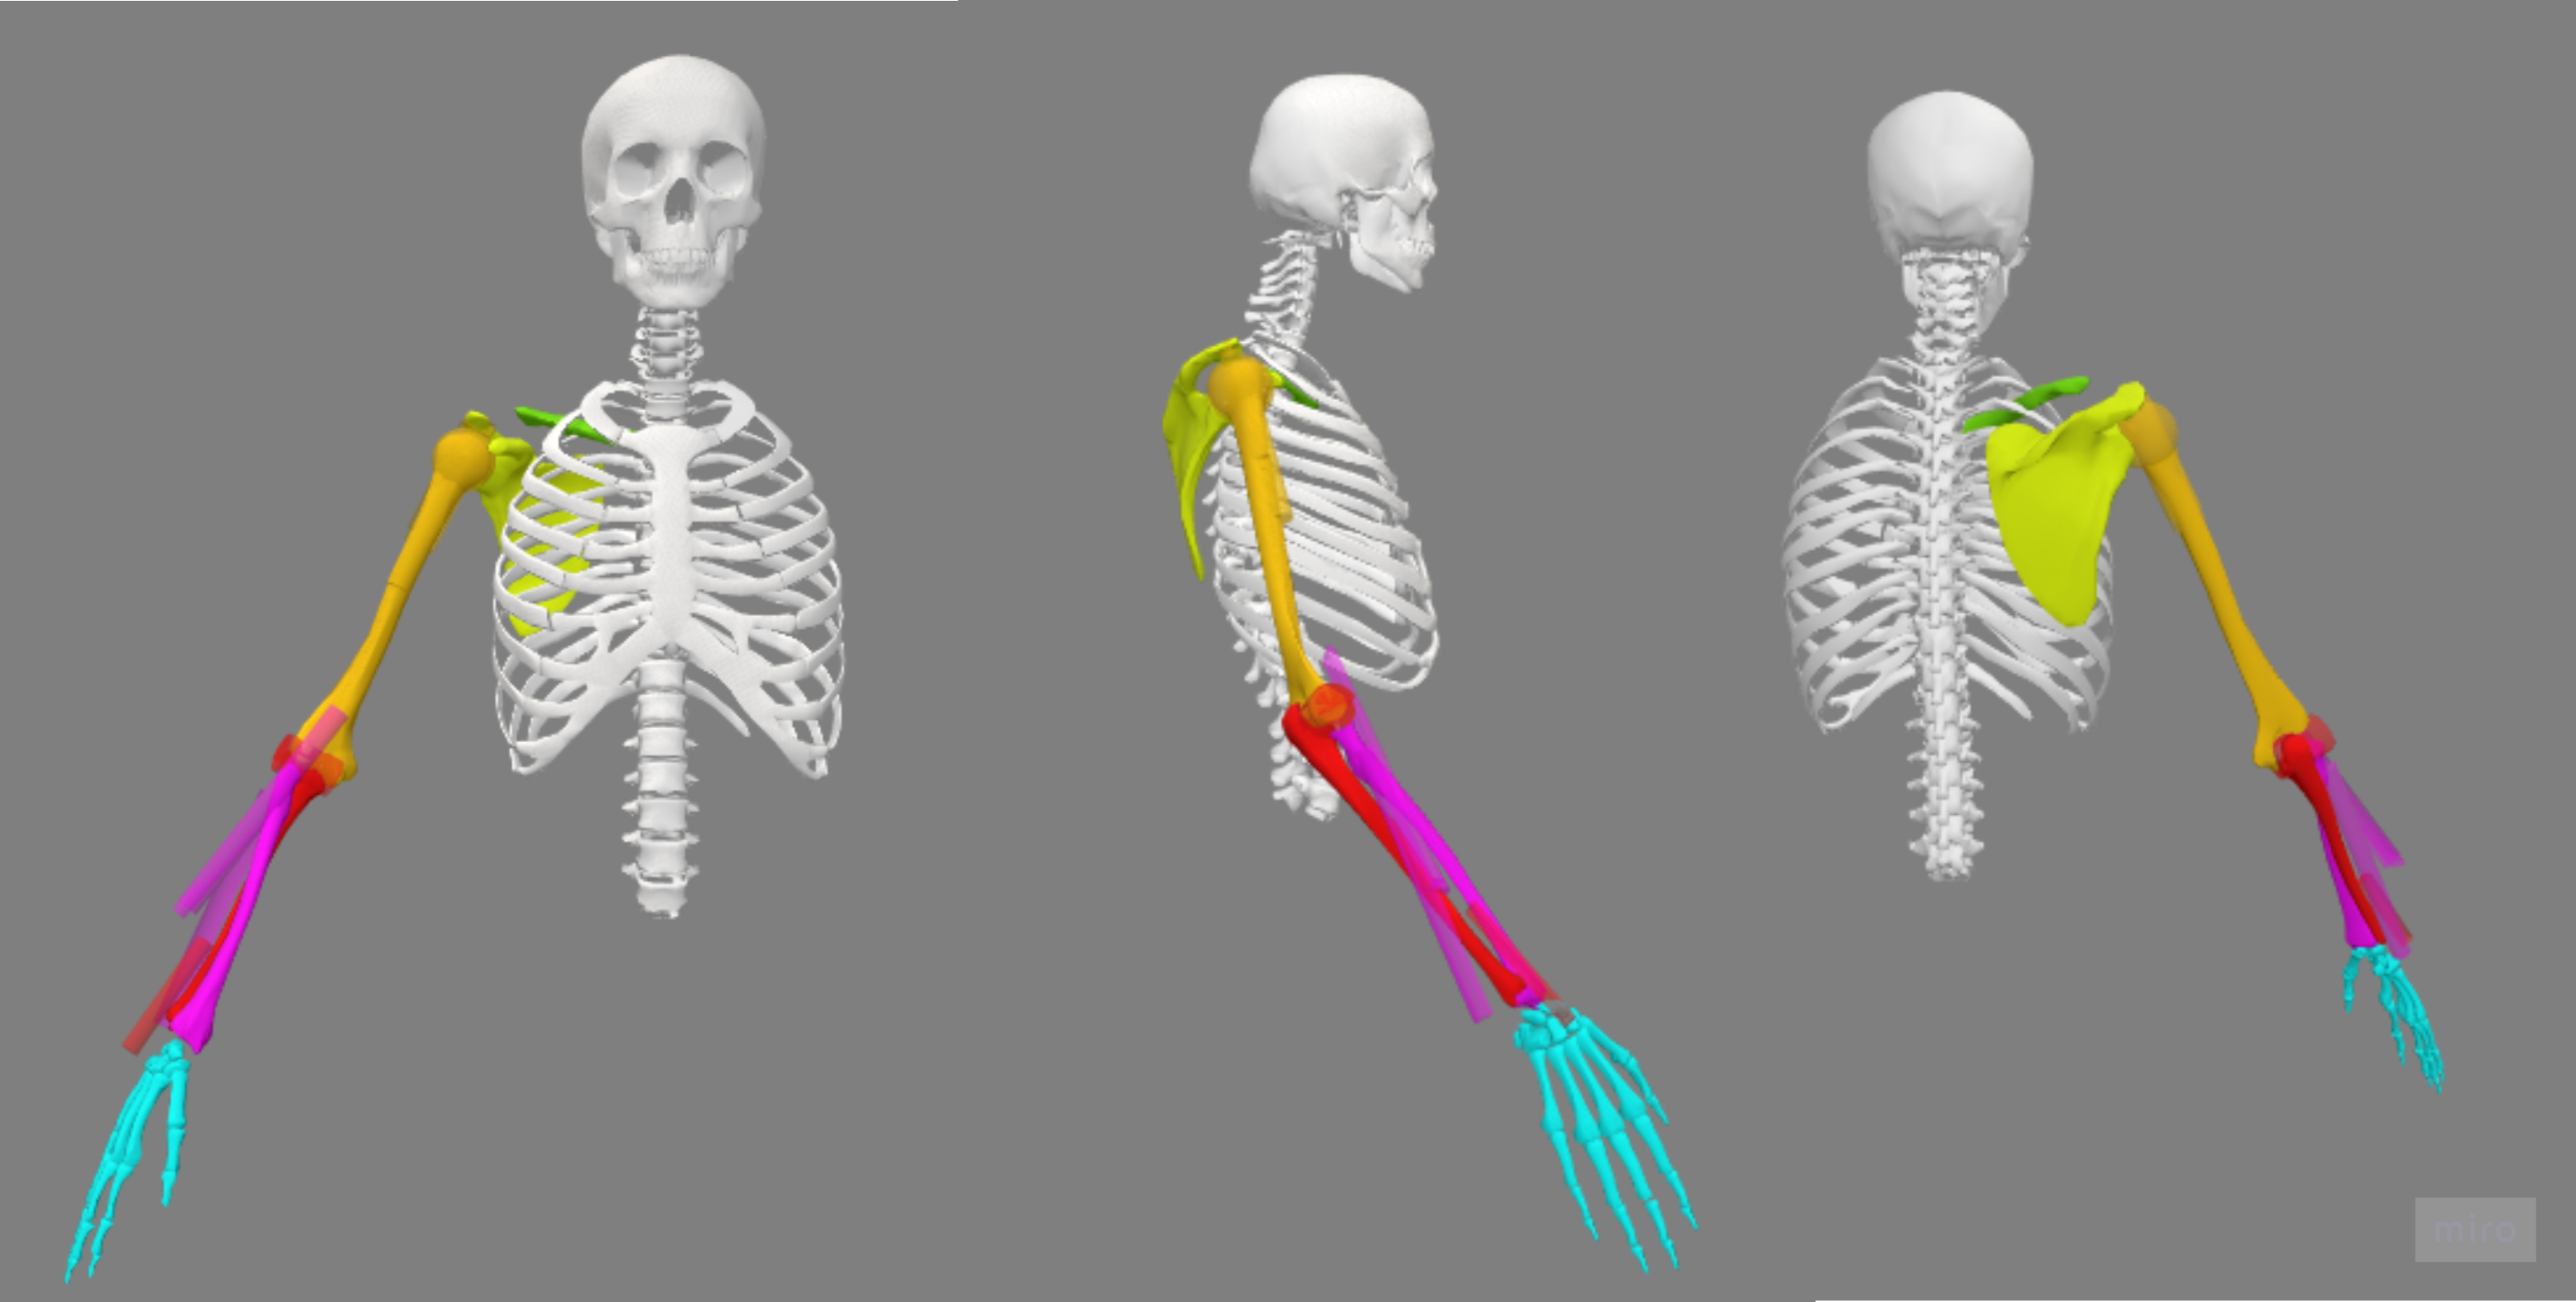
\includegraphics[width=0.7\textwidth]{Pictures/DAS/Links.png}
    \caption{Dynamic Arm Simulator 7 Links. Green: Clavicle, Yellow: Scapula, Orange: humerus, Red: Ulna, Purple: Radius, Blue: hand}
    \label{fig:links}
\end{figure}

\begin{itemize}
    \item \textbf{11 Degrees of Freedom}: These consist of 2 orthogonal hinges at specific joints, including the sternoclavicular, acromioclavicular and glenohumeral joints, elbow flexion-extension, and forearm pronation-supination (see Figure \ref{fig:measuring} for reference).  Initially, the model was focused on planar movement but was improved by adding independent control of the shoulder girdle. These additions allowed for more flexibility and stabilisation when designing the neuroprosthetic control algorithm \cite{RT3D}. The range of motion of the different DoFs is shown in Table \ref{table:11dof}.\newline
    
    Inspired by \cite{RT3D} throughout this project the arm configuration is described in 5 DoFs: plane of elevation, angle of elevation, internal rotation, elbow flexion and forearm pronation following the recommendation in \cite{ISB}. These angles were restricted in order to ensure correct wrapping of muscles in the model, the final values are show in Figure \ref{fig:5dof}.
\end{itemize}

\begin{figure}[h!]
    \centering
    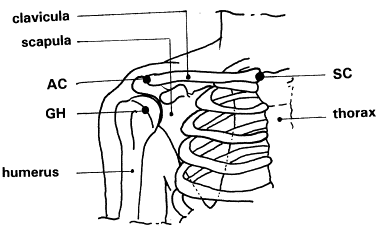
\includegraphics[width=0.6\textwidth]{Pictures/DAS/Joints.png}
    \caption{Shoulder mechanism of skeletal entities: thorax, clavicula, scapula and humerus; and the joints: sternoclavicular (SC) joint, acromioclavicular joint (AC) and glenohumeral joint (GH) \cite{Measuringmuscleandjoint}. }
    \label{fig:measuring}
\end{figure}

\begin{table}[h!]
\centering
\caption {\textit{Angular limits for each degree of freedom (in degrees)}: The arm mechanism consists of the following skeletal entities SC: Sternoclavicular joint, AC: Acromioclavicular joint, Gh: Glenohumeral joint, EL: Elbow, PS: Forearm Pronation and Supination.}
\label{table:11dof}
\begin{tabular}{ccc}
\hline
\textbf{Degree of Freedom} & \textbf{Min Angle (degrees)} & \textbf{Max Angle (degrees)} \\
\hline
SC y & -65.00 & -19.00 \\
SC z & 5.00 & 30.00 \\
SC x & 0.00 & 83.00 \\
AC y & 33.00 & 69.00 \\
AC z & -22.00 & 20.00 \\
AC x & -17.00 & 18.00 \\
Gh y & -170.00 & 175.00 \\
Gh z & -30.00 & 84.00 \\
Gh yy & -177.00 & 179.00 \\
EL x & 5.00 & 141.00 \\
PS y & 5.00 & 160.00 \\
\hline
\end{tabular}

\end{table}

\begin{figure}[h!]
    \centering
    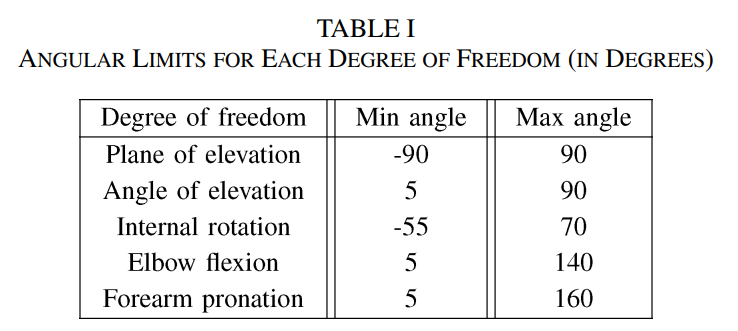
\includegraphics[width=0.7\textwidth]{Pictures/DAS/5dof.png}
    \caption{Angular limits for each degree of freedom (in degrees) for the arm configuration following \cite{ISB}. Table from \cite{RT3D}}
    \label{fig:5dof}
\end{figure}
\newpage
\begin{itemize}
    \item \textbf{22 Muscles and 138 Muscle Elements:} The real-time model consists of 22 muscles and muscle components in total. In order to accurately represent the mechanical line of action of each member, muscles are modeled using the fewest amount of parts possible. The table in Figure  \ref{fig:muscle_elements} displays the amount of elements utilized for each muscle as well as the degrees of freedom that each muscle crosses 
    
\end{itemize}

\begin{figure}[ht!]
    \centering
    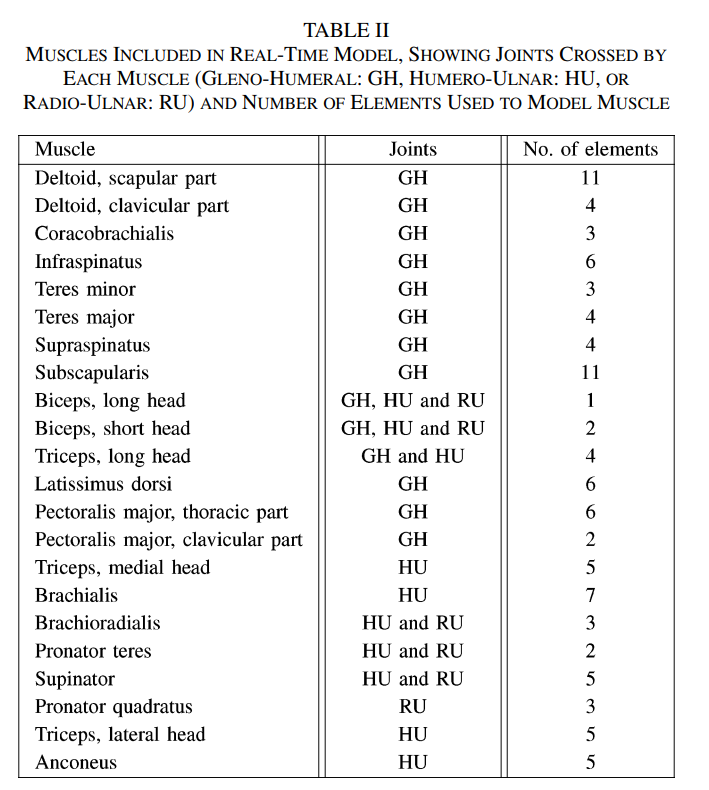
\includegraphics[width=0.7\textwidth]{Pictures/DAS/muscles_elements.png}
    \caption{Muscle elements and degrees of freedom crossed by the muscles. Table from \cite{RT3D}}
    \label{fig:muscle_elements}
\end{figure}

\newpage
\subsection{Musculoskeletal Dynamics}
% To do:: Explain the state variable and create a nomenclature table
The dynamics governing the musculoskeletal system must be thoroughly understood in order to research it. This analysis is divided into three interconnected components: multibody dynamics, muscle activation dynamics, and muscle contraction dynamics. Multibody dynamics allows us to represent the system as a collection of interconnected rigid or flexible bodies, focusing on the kinematic constraints that guide motion. Muscle contraction dynamics describes the complex interactions of muscle fibres and surrounding elements using the three-element Hill-type model, while muscle activation dynamics explores how neural signals translate into muscle actions.

The thorough analysis of the musculoskeletal dynamics is described in \cite{IMP}. In this section, a summary of each most relevant section is presented with a specific focus on the project's application.\newline


\subsubsection{State variables}\label{state}

It is necessary to define the state variables before examining the various dynamics of the multibody system.

The multibody model has 298 state variables. It is represented with the letter\textbf{ \textit{x}}:
\begin{itemize}
    \item 11 angles, $q$
    \item 11 angular velocities, $\dot{q}$
    \item 138 muscle contractile element (CE) lengths, $L_{CE}$
    \item 138 muscle active states, $a$
\end{itemize}

 
\subsubsection{Multibody dynamics}

Multibody dynamics is used to study the motion and forces acting on the musculoskeletal system as it is identified as a system composed of interconnected rigid or flexible bodies. 

Generalised coordinates are used to simplify the description of the system. As a result, the configuration of the system can be represented using the minimum number of coordinates to describe the position and orientation.  

Generalized coordinates, are often denoted by \textit{q}. They are a set of independent parameters that define the configuration of the system. In the DAS \textit{q} represents the 11 joint angles. 

The equations of motion for a multibody system can be expressed in the following matrix form (\cite{Siciliano2009}):
\begin{equation}
    M(q)*\Ddot{q} + B(q,\dot{q}) = \tau
    \label{eq:MBD}
\end{equation}

Where,
\begin{itemize}
    \item $\ddot{q}$ is the vector of generalized accelerations
    \item $M(q)$ is the mass matrix that describes the inertia of the system. It relates the acceleration of \textit{q} to the generalized forces.
    \item $B(q,\dot{q})$ is the matrix that describes Coriolis and centrifugal forces that arise from the motion of the bodies in the system. Moreover, it contains gravity and other passive forces.
    \item $\tau$ is the generalised force vector. In the case of DAS it represents the forces generated by muscles according to the muscle contraction and activation dynamics. 
\end{itemize}

Forward dynamics is used to predict the motion of a multibody system based on its initial conditions and known forces. As a result Equation \ref{eq:MBD} is solved to the generalized accelerations $\ddot{q}$.

\begin{equation}
    \ddot{q} = M(q)^{-1}(\tau - B(q,\dot{q}))
\end{equation}

The inverse of the mass matrix, $M$, is a critical component, as the simulation will not be possible if its singular. This singularity is quite common in musculoskeletal systems due to small mass and moment of inertia of body segments.

Moreover, elements of $B$ can present high stiffness and damping, leading to high eigenvalues of the Jacobian matrix that correspond to fast-changing components of the system. These high stiffness and high damping lead to oscillatory behaviours within the system. The presence of stiffness originates from the ligaments and tendons having highly nonlinear mechanical properties (zero stiffness when unloaded, high stiffness when maximally loaded).

To counteract the stiff system, standard numerical methods, such as Euler method, require small time steps.


\subsubsection{Muscle contraction dynamics} \label{musclecontraction}

The muscle contraction dynamics is based on the three-element Hill-type model. It represents the muscle fibers (CE: contractile element), the tendon and force transmitting tissue (SEE: series elastic element), and the passive elastic tissue surrounding the muscle fibers (PEE: passive elastic element). 
\begin{figure}[h!]
    \centering
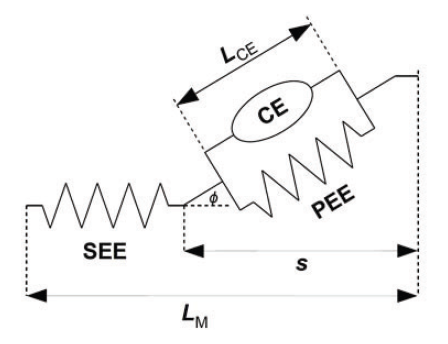
\includegraphics[width=0.4\textwidth]{Pictures/DAS/Hill-Type_MuscleModel.png}
    \caption{Three-element muscle model. CE: contractile element, SEE: series elastic element, PEE: parallel elastic element, Pennation angle $\phi$: Angle between the muscle fiber in the CE and the line of action of the muscle, $s$ state variable for the muscle contraction dynamics \cite{IMP}}
    \label{fig:Hill-type}
\end{figure}

The contractile force is calculated by the multiplicative interaction of the maximal isometric force, the activation, the fiber length and the fiber length velocity, respectively represented in the formula below:
\begin{equation}
    F_{CE} = F_{max}*a*f_{FL}(L_{CE})*f_{FV}(\dot{L_{CE}})
\end{equation}

The series and parallel elastic elements are represented by passive force-length relationships.
\begin{equation}
    F_{SEE} = f_{SEE}(L_{M}-L_{CE}*cos(\phi))
\end{equation}
\begin{equation}
    F_{PEE} = f_{PEE}(L_{CE})
\end{equation}

The force balance equation following Figure \ref{fig:muscle_elements} is equal to:
\begin{equation}
    (F_{CE}+F_{PEE})*cos(\phi) - F_{SEE} = 0
    \label{eq:MCD}
\end{equation}

The differential equation for the state variable $L_{CE}$ is defined by Equation \ref{eq:MCD}.  
\newline
\subsubsection{Muscle activation dynamics}

The nervous system sends a neural excitation $u(t)$ as a control signal to the muscle that changes the activation through a first-order non-linear activation-deactivation process. This is because the activation $a$, also called the \textit{ active state} cannot be directly controlled by the nervous system. The  muscle activation of a muscle, $a$, is formulated as:

\begin{equation}
    \dot{a} = (u-a)(c_{1}u + c_{2})
    \label{eq:MAD}
\end{equation},

where $c_{1} + c_{2}$ is the rate constant for activation and $c_{2}$ is the rate constant for deactivation, typically in the range of 20-50 $s^{-1}$ \cite{IMP}.

Combining Equation \ref{eq:MBD}, Equation \ref{eq:MCD} and Equation \ref{eq:MAD} an implicit state equation for musculoskeletal dynamics can be formulated.  

\subsection{Forward Dynamics for implicit state equation}\label{forward}

The forward dynamic simulation of the musculoskeletal system model is a complex process that involves determining the state trajectory $x(t)$, starting from an initial state at $t = 0$ and using a control function $u$ that contains the neural excitations for all muscles. 

As mentioned in section \ref{state} the state vector $x$ is equal to:

\begin{equation}
    x = (q,\dot{q},s,a)^T
\end{equation}

$q$ and $\dot{q}$ for each degree of freedom and $s$ and $a$ for each muscle.

All dynamic equations for the model, which include equilibrium of forces and activation for muscle control (Equation \ref{eq:MBD}, Equation \ref{eq:MCD} and Equation \ref{eq:MAD}) are combined into one single equation in terms of the state vector $x$ and control input $u$.

\begin{equation} \label{eq:implicit}
    f(x,\dot{x},u)=0
\end{equation}

This equation is implicit as there are relationships among the variables. In contrast with explicit formulation, they can not be solve directly for each variable. Solving this implicit equation in a conventional can be hard to solve numerically. This usually requires small steps in simulation, making it time-consuming, computationally expensive and less accurate.

The DAS uses an alternative approach where by leaving the equation in its implicit form is possible to calculate the Jacobian of $f$ with respect to $x$, $\dot{x}$ and $u$. \cite{IMP}.

To predict how muscles and joints mover time based on an initial condition and neural excitations controls, the differential algebraic equation (DAEs) must be solved (Equation \ref{eq:implicit}). 

For real time simulation, the DAS uses Rosenbrock method as it requires quick and predictable computations. The Rosenbrock method is a numerical technique used to solve ordinary differential equations (ODEs). The ordinary differential equations describe how the arm motion changes over time. The Rosenbrock methods involves predicting the state at the next time step. It iterates until finds the right guess. The main advantages of Rosenbrcok is that it produce realistic values if the Jacobian matrices are known.

The DAS implements a first order method with constant step size $h$. This means that if the the step size is halved, the error will also be halved. 
\begin{equation} \label{eq:rosenbrock}
 \begin{aligned}
    \Delta x = (\frac{\partial f}{\partial x} + \frac{1}{h}\frac{\partial f}
    {\partial \dot{x}})^{-1}(\frac{\partial f}{\partial \dot{x}}\dot{x}_n - f(x_n, \dot{x}_n, u_n) - \frac{\partial f}{\partial u}*(u_{n+1} - u_{n}))\\
    x_{n+1} = x_n + \Delta{x} \\
    \dot{x}_{n+1} = \frac{\Delta{x}}{h}
\end{aligned}
\end{equation} \newpage

\subsection{Functionalities}

The DAS can be downloaded from the simTK.org website (\href{https://simtk.org/projects/das}{https://simtk.org/projects/das}). It includes the \textbf{main MEX file}, some files to test the correct functionality and installation of the simulation environment and a basic manual for understanding its different functionalities. 

\subsubsection{Loading the model}

During the initialization the MEX functions reads in the parameters from the model. When initializing the model the 13 joints and 138 muscle elements are loaded.

\begin{lstlisting}[style=Matlab-editor]
load model_struct;
das3('Initiliaze',model);
\end{lstlisting}
\subsubsection{Joint Moments}
The input is the states of the model and the output presents the moment of the arm for each degree of freedom (N m)
\begin{lstlisting}[style=Matlab-editor]
moments = das3('Jointmoments', x) %(ndof x 1)
\end{lstlisting}

\subsubsection{Muscle Forces}
The input is the states of the model and the output presents the forces of the arm for each muscles (N)
\begin{lstlisting}[style=Matlab-editor]
forces = das3('Muscleforces', x)
\end{lstlisting}

\subsubsection{Muscle Length and SEE Slack}
The length of each muscle (meters) and the slack length of series elastic element (m) are given using the \textit{'Musclelengths'} and \textit{'SEEslack'} functions respectively. 

When a muscle contracts, it shortens its length to produce force. Before being applied to the load, this force passes via the series elastic element (SEE). The SEE is in a slack or non-stretched state when a muscle is in rest and not exerting any force. Because the SEE is not applying any further tension to the muscle fibers at this time, the length of the contractile element (CE) is equal to the length of each muscle fiber. However, when the force is transmitted through the SEE when the muscle contracts and generates force, the SEE begins to stretch and the CE shortens. 

In general, the CE length is equal to the length of each muscle fibre when the muscle is relaxed and does not generate any force. When a force is applied, i.e., during muscle contraction, the CE shortens and the SEE stretches, enabling efficient force transmission to the load. This is why to calculate the correct length of the muscle in an initial state where the muscle is contracted, the CE value is equal to the formula below.

\begin{equation}
    LCE = length - SEEslack \label{LCE}
\end{equation}

The function below initializes the muscle values for the state correctly when knowing only the angle values for the different degrees of freedom.\newpage

\begin{lstlisting}[style=Matlab-editor]

function x = initialize_state(position, nstates, iLce)
    x=zeros(nstates,1);
    LCEopt=das3('LCEopt');
    lengths = das3('Musclelengths', x);    % only the first 11 elements of x (the joint angles) will be used
    SEEslack = das3('SEEslack');
    Lce = (lengths - SEEslack);
    x(iLce)=Lce;
    x(1:11)=position;

end
\end{lstlisting}

Go to Section \ref{musclecontraction} for more information on the three-element model used to model muscle contraction dynamics. \newline

\subsubsection{Dynamics}
This function is to evaluate the dynamics of the model in the implicit form f(x,$\dot{x}$,u) = 0.
The inputs are:
\begin{itemize}
    \item x (nstates x 1) : the model states.
    \item $\dot{x}$ (nstates x 1): the derivatives of the state of the model.
    \item u (nmus x 1): muscle excitations.
\end{itemize}

Some optional inputs include
\begin{itemize}
    \item M (5x1): moments applied to the thorax-humerus YZY and the elbow flexion and supination axes.
    \item exF (2x1): external vertical force of amplitude exF(2) applied at exF(1) meters from the elbow.
    \item handF (3x1): force applied to the center of mass of the hand. The positive value of handF (1) represents the lateral movement far from the thorax, the positive value of handF (2) represents the upward movement, and the positive value of handF (3) represents the posterior movement.
\end{itemize}

The outputs are as follows:

\begin{itemize}
    \item f (nstates x 1): dynamic imbalance.
\end{itemize}

Optional outputs include
\begin{itemize}
    \item $\frac{\partial f}{\partial x}$ (nstates x nstates): Jacobian of f with respect to x.
    \item $\frac{\partial f}{\partial \dot{x}}$ (nstates x nstates): Jacobian of f with respect to $\dot{x}$.
    \item $\frac{\partial f}{\partial u}$ (nstates x nmus): Jacobian of f with respect to u.
    \item qTH (3x1): angles between the thorax and humerus (YZY sequence). This angles are calculate following the standardization on \cite{ISB}
\end{itemize}
\begin{lstlisting}[style=Matlab-editor]
[f, dfdx, dfdxdot, dfdu, ~,~,qTH] = das3('Dynamics',x,xdot,step_u,M,exF,handF);
\end{lstlisting}

The das3step function is used to calculate the next time step following the Rosenbrock method (Equation \ref{eq:rosenbrock}) previously explained in Section \ref{forward}.

\begin{lstlisting}[style=Matlab-editor]
function [x, xdot, step_u, qTH] = das3step(x, u, tstep, xdot, step_u, M, exF, handF)
    [f, dfdx, dfdxdot, dfdu, ~,~,qTH] = das3('Dynamics',x,xdot,step_u,M,exF,handF);
    
	% Solve the change in x from the 1st order Rosenbrock formula
	du = u - step_u;
	dx = (dfdx + dfdxdot/h)\(dfdxdot*xdot - f - dfdu*du);
	xnew = x + dx;
	
	% update variables for the next simulation step
	xdot = dx/h;
	step_u = u;
end
\end{lstlisting}\label{matlab:das3step}


\subsubsection{Visualization}

The model can be visualised in OpenSim as shown in the image below. However, for user-friendliness the DAS presents a function named \textit{das3stick(x,model)}. The inputs are the model state and the Matlab model structure, and it outputs a Matlab figure with a more simplified drawing of the model. 
\begin{figure}[h]
    \centering
    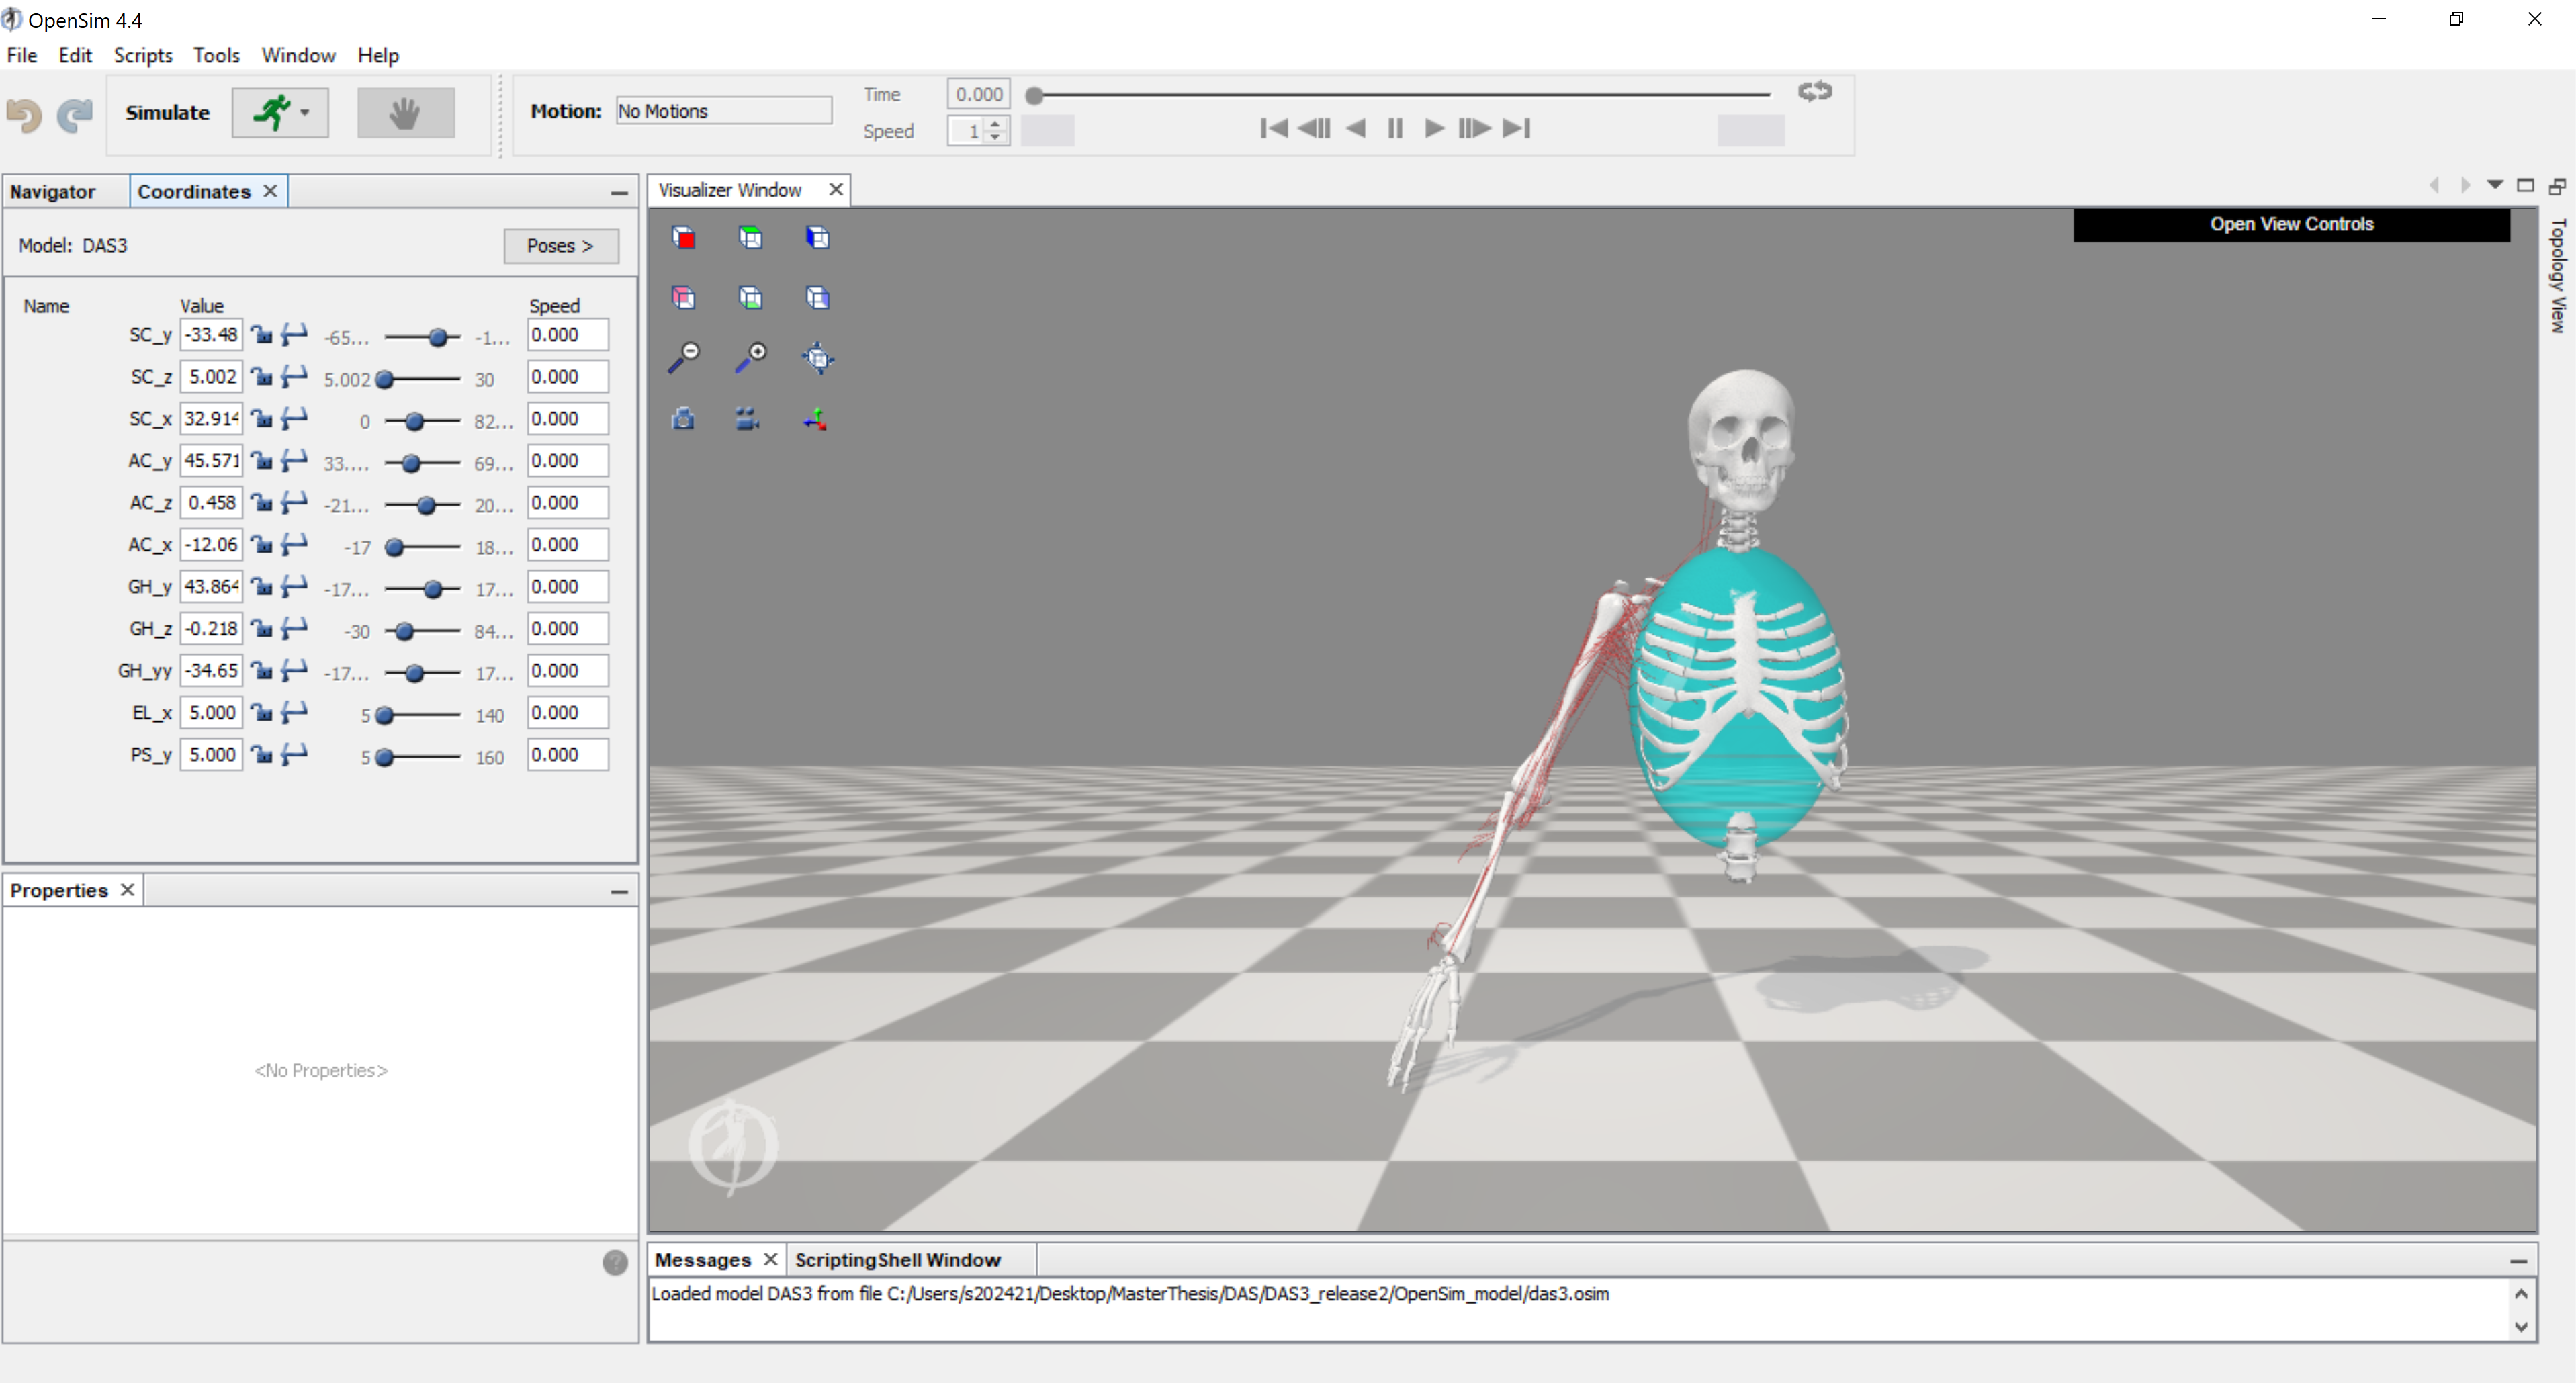
\includegraphics[width=0.7\textwidth]{Pictures/DAS/OpenSimModel.png}
    \caption{Open Sim DAS}
    \label{fig:OpenSimDAS}
\end{figure}

\begin{lstlisting}[style=Matlab-editor]
    das3stick(xneutral,model);
 \end{lstlisting}

 Output of the \textit{das3stick}

 \begin{figure}[h]
    \centering
    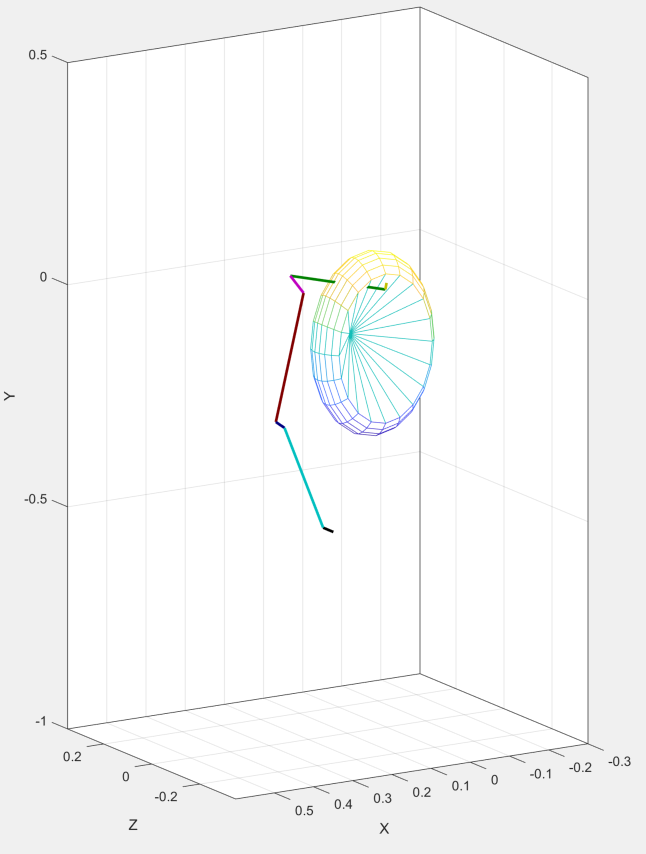
\includegraphics[width=0.4\textwidth]{Pictures/DAS/das3stick.png}
    \caption{Matlab Visualization Output}
    \label{fig:das3stick}
\end{figure}

The \textit{das3stick} function utilizes the \textit{'Visualization'} functionality that outputs a 13x12 matrix $d$ that contains the orientation matrix and position vector information for each bone.

\begin{lstlisting}[style=Matlab-editor]
    d = das3('Visualization',x);   
    p = d(j,1:3)';					% position vector of bone
    R = reshape(d(j,4:12),3,3)';	% orientation matrix
 \end{lstlisting}

